\chapter[\'Etude en clinique]{\'Etude clinique}
Utilisation du test
  d'écoute en clinique psychiatrique
( comme précédemment annoncé, cf.Zwicker, (distorsion)module:
testtomatis)



En général, dans les milieux psychiatriques, la musicothérapie est de plus en plus
intégrée, comme c'est le cas dans notre étude.
En effet, l'interrogation principale du travail s'axe sur la nécessité
de
vérification de l'amélioration de
la capacité d'écoute chez le
patient, après un travail musicothérapeutique.



*6.1.cf. Concept piagetien de l'\textit{assimilation} majorante (
parallélisme avec une amélioration cognitive dite majorante)
amélioration perceptuelle implique tout le procédé, va toucher tout le
système, développement de l'intelligence, pas que dans la logique,mais
par l'art, 
processus d'accomodation.


*Le thérapeute va améliorer
Lien avec Piaget

\section{Cadre de travail, population et méthodologie}

 La clinique privée (Privatklinik)
de Meiringen (BE) est  principalement spécialisée en
addictologie avec problèmes d'alcool et de toxicodépendance, couvrant aussi les aspects dépressifs
et les
burnouts.


Elle dispose d'une capacité de
195 lits, et le temps de séjour fluctue de 3 à 6 semaines ou plus, en
fonction de la participation des assurances.

Actuellement, en plus de l'administration et l'intendance, les 33
médecins et psychiatres, sont
accompagnés par 177
soignants, dont infirmiers psychiatriques, aide-infirmières, physio et
ergothérapeutes, 
psychologues et intervenants en \textit{thérapies
créatives }, comme l'art-thérapie, thérapie
corporelle, zoothérapie (chien/ cheval),  ateliers de créativité --
bois et terre --,  les textiles et la\textbf{ musicothérapie} (deux
personnes, respectivement à 90 et 10 pour cent).


\textbf{Demander organigramme}. proportion exacte
dont la souscrite à titre de 10 pour cent.
Pour\textbf{ Powerpoint}


(-OH*:  le radical hydroxile, oxydrile de la molécule éthylique)




L'\textbf{échantillonnage} fortement conditionné par les contraintes
institutionnelles, comme les interruptions prématurées de séjour, les rendez-vous
 médicaux superposés, l'impossibilité de participation physique et/ou
 psychique, les remplacements disparates et hétéroclites de ma
 collègue, l'emploi à
 temps partiel, a été restreint  par le choix d'un nombre limité de
 patients (Nb=29).
Une autre contrainte de nature extra-institutionnelle allant dans le
même sens réside dans l'éloignement géographique.

En synthèse:
 \begin{itemize}
 
 \item \textbf{Nombre total de personnes}: Nb= 29 
\item\textbf{Genre et âge de la population étudiée:}  19 hommes et 10 femmes, de 25 à 72
  ans dont l'âge moyen est de 48 ans. x= 48.
 \item\textbf{Pathologies}: burnout, dépendances, dépression.
 \item \textbf{Nombre total de séances} par personne en
   musicothérapie= 4 ;   \textbf{mu}=1/semaine;  
 \textbf{t}= 50--60 min, période = 3 -- 4 semaines.
\end{itemize}




 mu en grec
\section{Méthodologie et  ensemble des démarches}






Obtenu l'aval de la part de la direction de la
clinique pour cette étude,  le personnel soignant et l'ensemble des membres des
thérapies créatives ont été informés verbalement et par écrit, texte
destiné aussi aux
patients\footnote{ \emph{Information für Mitwirkende an der klinischen
  Studie\  ``Evaluierung des aktiven Hörvermögens" }
}  \footnote{Cf.Annexe D.}, expliquant le projet d'une étude sur l'écoute, ainsi que
sur l'hypothèse de sa transformation dans un processus thérapeutique, 
avec ou sans musicothérapie.

La proposition effectuée par l'intermédiaire de la musicothérapeute  Regula Lehman \footnote{Regula
  Lehmann, musicothérapeute  à 90\%  à la clinique de Meiringen.} dans un
court entretien individuel, a donné suite à  la signature de la 
feuille de consentement  officiel de leur libre 
accord. \footnote{\emph{``Eine schriftliche Einbewilligung zum
    Test"}.}

Après ces prémisses, l'étude commence véritablement avec l'application du test
audiométrique suivie du questionnaire qualitatif.

\subsection{Déroulement de l'étude:}

Les tests et questionnaires  ont été réalisés de juin à octobre 2017 sur une durée de quatre semaines, correspondant au séjour moyen.

\textbf{Type de thérapie: la musicothérapie}: réceptive  et active
(mélangées).

Les autres thérapies mentionnées plus haut ont pu être suivies en parallèle par les deux
groupes concernés mais ne font parties de l'analyse comparative.

 La thérapie Tomatis ---avec l'écoute sous casques spécifiques et
 musiques modifiées--- n'a intentionnellement pas été utilisée et
 volontairement exclue de notre travail.



\textbf{Les groupes}

Le groupe groupe expérimental, G M., comporte 21 patients, avec 15 hommes et 6
femmes.
Le groupe G C., groupe de contrôle, comporte 8 patients, 4 hommes et
4 femmes.






 
 
 

\section{Instruments de mesure: le WHO QOL - Bref et le test d'écoute}
 Nous redonnons quelques précisions sur le WHO QOL-Bref mais ne
 reviendrons pas sur le test d'écoute, suffisamment décrit plus haut. Il a été
 utilisé pour constater une modification au cas où celle-ci
 n'apparaitrait pas avec le test d'coute.

 \subsection{Le WHO QOL - Bref:  World Health
   Organisation Quality of Life Assessement }
 
Le  WHOQOL-Bref sert à évaluer la qualité de vie des patients. C'est une échelle
d'auto-évaluation subjective qui évalue la santé mentale, le
bien-être, l'environnement et les relations sociales.
Il s'agit ici de la version courte  la plus récente (2004) du questionnaire
 WHOQOL-100 datant de 1998, version issue du Programme sur la santé
 mentale de l'
Organisation mondiale de la santé de Genève. Il y a 26 questions
courtes, dont un item concernant la qualité de vie globale
auto-évaluée par le sujet, un item évaluant la santé générale perçue
et les 24 autres se répartissent selon les 4 domaines suivants:  
: physique, psychologique, relations sociales et environnement.
\begin{enumerate}
\item  Le domaine de la perception physique (7 items) comprend l' activité quotidienne// la dépendance et/ou l'assistance médicale// la fatigabilité, l'énergie//la mobilité// la douleur// le sommeil// la capacité de travail//
	
\item Le domaine psychologique (6 items):  image de soi, apparence// ressentis positifs et négatifs// estime de soi// spiritualité, croyances personnelles, religion// mémoire et concentration, apprentissage, pensée.
		
\item Le domaine des relations sociales (3 items) : relations personnelles// soutien social// vie sexuelle.
			
\item Le domaine de l'environnement (8 items) :
                         l'environnement domestique et physique
                         (pollution, bruit, trafic, climat)// la
                         situation financière//  la liberté, la
                         sécurité physique et morale//
                         l'accessibilité et qualité de la santé// les
                         opportunités de détente, loisirs, accès aux
                         informations// logement et transport// 
\end{enumerate}
		
	

Les questions varient selon sa propre perception, telle la satisfaction
au sujet de son  sommeil, de sa vie relationelle, sexuelle, de
l'opinion de que l'on a sur soi,  `` Êtes-vous satisfait de
vous-même?'' , ``Acceptez-vous votre apparence physique?''ou si le patient éprouve souvent des sentiments négatifs
et/ou s'il a assez d'énergie dans la vie de tous les jours.
La cotation se fait sur 4 types d'échelles de réponses en 5 points
permettant l'évaluation de l'intensité, la fréquence, la capacité, l'évaluation.
de 1 à 5.
Le patient le remplit avec ou sans aide du
thérapeut lors de chaque test
d'écoute. La durée variera de 3 à 10 minutes en
moyenne. 
Nous avons utilisé et fait en parallèle le test WHOQO-Bref pour avoir une variable supplémentaire pour confirmer en
parallèle supposée de l'action de la musicothérapie sur une éventuelle modification de l'écoute.


        	
 \subsection{Technique d'intervention:}


       
\begin{itemize}
\item Le groupe G M., avec musicothérapie : un
          test avant leur prise en charge en musicothérapie; avec un questionnaire
          WHOQOL.
          
\item Un 2\ieme\ test et un questionnaire WHOQOL : après 4 semaines de
          clinique.
          
\item Un groupe G C.  sans musicothérapie, (contexte idem)
	toujours dans le même contexte, c.à.dire en clinique, avec le suivi et les mêmes protocoles que l'autre groupe. Un premier test avant
 puis un deuxième test, avec les questionnaires WHOQOL, après 4 semaines. 
\end{itemize}

\textbf{ Par ordre chronologique:}
 
\begin{enumerate} 
   \item Un test d'écoute, un entretien et un questionnaire
        WHOQOL pour les deux groupes.
    \item Séances de musicothérapie, actives ou réceptives (1x par
        semaine) pour GM.
    \item Deuxième test d'écoute, entretien et questionnaire
          WHOQOL pour les deux groupes.
\end{enumerate}

	
	
	\textbf{Durée des tests} : Chaque test d'écoute a une durée  moyenne de
        70 à 90 minutes par patient. Pour chacun, nous avons donc réalisé
        en tout au minimum 2h30 de tests d'écoute sur lesquels
        s'ajoute un
        entretien (2x15') à chaque fois.

        
        Le questionnaire WHOQOL (2x10')  a été remplis par les
        patients avant le début du séjour en clinique et après, lors
        de leur sortie.
        
       
      
      \paragraph{Résultats, nombre de tests réalisés:}

        
     Nous avons réalisé en tout 44 tests d'écoute et 25 questionnaires 
     WHOQOL-Bref.
     
     Sur les tests d'écoute: il y a 35 tests d'écoute (1°+2°=
     avant/après), valides, qui nous permettront de faire une
     comparaison.

     
     21 personnes ont fait le 1°test et 8 d'entre-elles ont fait le
     2°test.

     C.à.dire: 8x1° et 8x2°
     -8 personnes avec pour chacune 2 tests( avant/après), soit  un
     total de 16 tests d'écoute pour le groupe d'expérimentation, en musicothérapie
     1°: GM= 21
     2°: GM= 8
     
     -8 personnes avec un total de 15 tests d'écoute pour le groupe de contrôle, sans suivi en 
     musicothérapie,c.à.dire: 8x1° et 7x2°
     1°: GC= 8
     2°: GC= 7

     
           Sur les 25  questionnaires WHOQOL remplis:
           
     - 10 questionnaires (8x1°) et (2x2°) pour GM.
     1°: GM= 8           //             2°: GE= 2
     - 15 questionnaires (8x1°) et (7x2°) pour GC.
    
     1° GC= 8             //            2°: GC= 7
     
     
    
 
     
          
 
 
 	
 	
       

 	
 	\section{Un graphique: déroulement de l'étude avec un groupe
          de contrôle et un groupe d'intervention}





                                      Patients souffrant de dépression, burnout
                                               en séjour dans la
                                               clinique, répartis en
                                               deux groupes.
                                               Nous avons conscience
                                               d'avoir mélangé deux
                                               symptomatologies qui
                                               toutefois paraissent
                                               sous-tendues par les
                                               mêmes mécanismes et
                                               s'exprimant par une
                                               humeur négative.

\begin{figure}
\centering
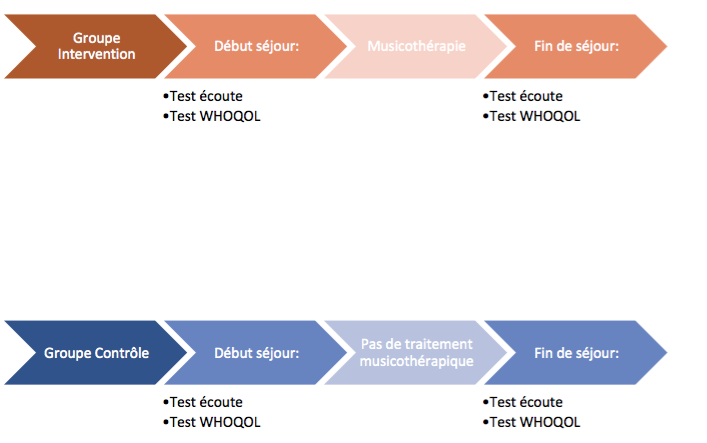
\includegraphics[width=0.7\linewidth]{images/Groupecontrole.png}
\caption[Schéma du déroulement]{Déroulement de l'étude avec GM (intervention) et GC}
       
\label{groupecontroleimage1}
\end{figure}

\begin{figure}
\centering
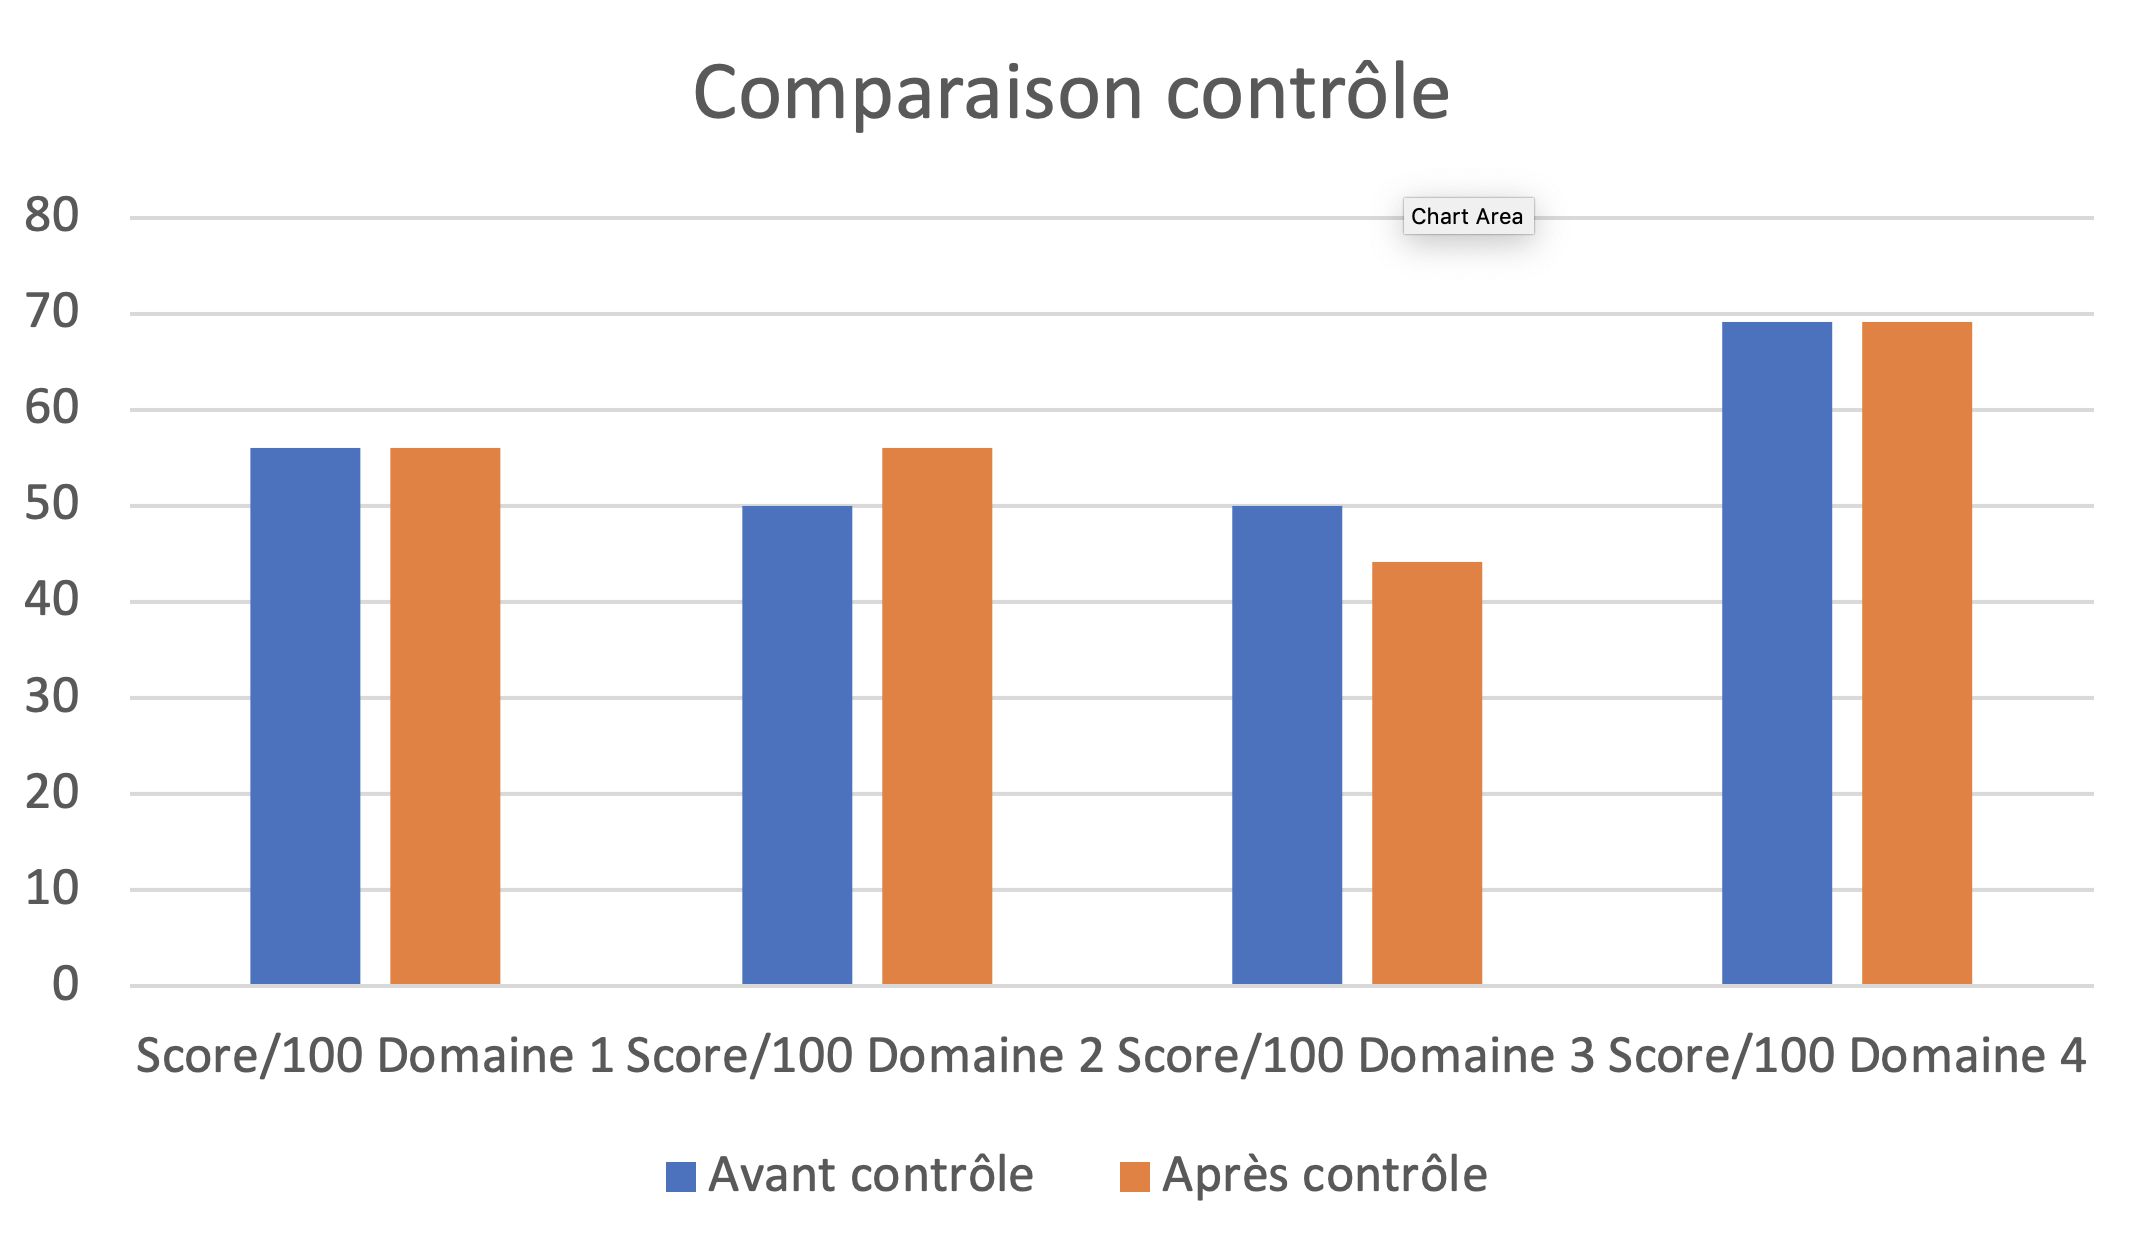
\includegraphics[width=0.7\linewidth]{images/Compcontrole.png}
\caption[Schéma du déroulement]{Comparatif des questionnaires 1°+2°
  WHOQOL pour GC}
       
\label{groupecontroleimage1}
\end{figure}

\begin{figure}
\centering
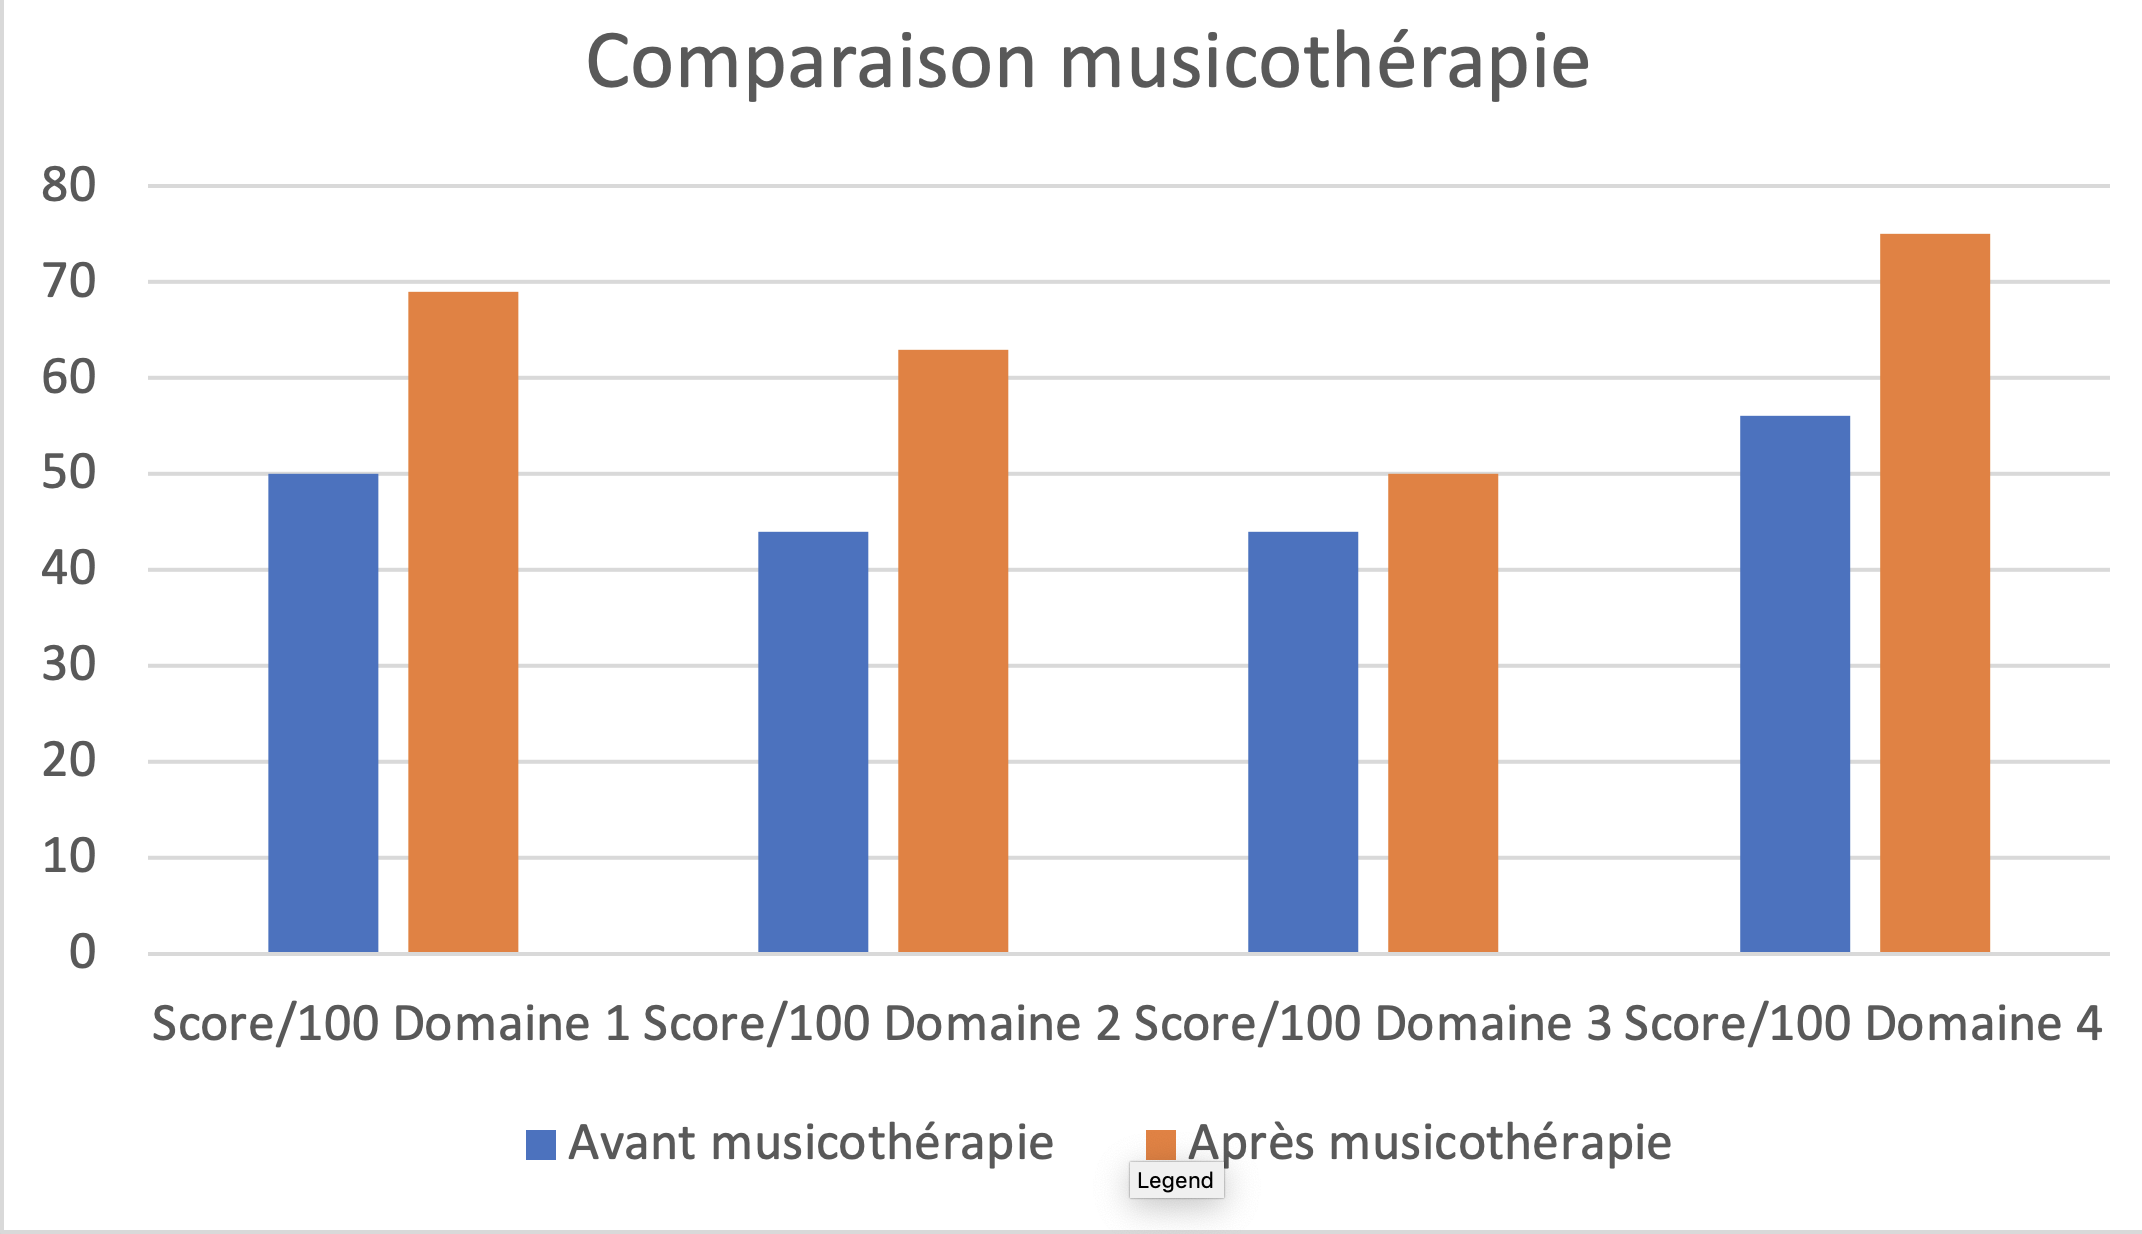
\includegraphics[width=0.7\linewidth]{images/Compmusico.png}
\caption[Schéma du déroulement]{Comparatif des
         questionnaires 1°+2° WHOQOL pour GMusic.}
       
\label{groupecontroleimage1}
\end{figure}

                                             
\subsection{Constatations: }
En vue de la taille réduite des échantillons, il n'est pas
pertinent de se lancer dans une analyse purement
quantitative. Néanmoins, nous 
allons prendre en compte les seuils auditifs que nous  alierons à une étude
qualitative ( interprétation psychologique) basée sur 
des données relevables avec les
graphiques -- les trois zones de fréquences--issus des tests d'écoute.


Les données quantitatives observables dans ces graphiques semblent aller dans le
sens de  l'étude faite par le
CNRS (cf.p.19J.P.) réalisée à partir des seuils auditifs, à savoir
les patients souffrant de dépression semblent souffrir d'un
appauvrissement de fréquences caractéristiques.

Il s'agira  ainsi d'une étude dite de type  ``aléatoire'' mixant le  quantitatif  et le qualitatif.

(Perspective: il aurait été judicieux de passer une échelle de
dépression afin d'objectiver le degré de sévérité des dépressions.)

Voici l'illustration avec un test
d'écoute sur un sujet dépressif que nous avons réalisé lors de notre
étude en clinique: la
chute des fréquences dans des zones de fréquences élevées est
clairement visible.\footnote{Cf.Fig.3.1}
 \begin{figure}
	\centering
	\includegraphics[width=0.7\linewidth]{images/courbesdeepressif.jpg}
	\caption{Courbes dépressif}
	\label{fig:courbes du dépressif}
      \end{figure}

  \section{La dépression, le burnout et leur expression
    musico--physico--psychologique:}

  
En nous référant aux
caractéristiques décrites de sujets dépressifs (cf.p.10), notamment avec le test
et échantillon de Hamilton (cf.p.19), nous avons tenté de dresser un portrait
du dépressif avec les réactions physiologiques et psychologiques
  en les mettant en relation avec les trois zones relevées évoquées.

\paragraph{Descriptif d'un dépressif selon les zones d'nterprétation:}



\begin{itemize}
  	\item Zone 1 :  Le rythme cardiaque: un stress intense va modifier le rythme
  du corps en augmentant ses fréquences. La respiration deviendra
  rapide. Il va s'en suivre une modification des perceptions
  extérieures. Une sensibilité particulièrement accrue aux bruits et
  aux sons peut en découler et être vécue comme une
  atteinte physique et psychique insupportable.
  Le changement de posture et d'attitude corporelle sont
notables (affaissement) et la perte d'énergie physique considérable ( épuisement).


 	\item Zone 2: La qualité de la voix: changement de la qualité du timbre de la
 voix et de l'émission verbale.
  La voix se caractérise par son volume, son timbre, sa mélodie et son langage. 
 	
 	De manière très appropriées, nous pouvons faire ainsi le
        descriptif général de la voix d'un patient dépressif ou
        stressé avec: le volume, le timbre, la
        mélodie, le langage: 
 	\begin{enumerate}
 		\item le volume : basse intensité, faible dynamique
 		\item la mélodie : monotone, sans modulation
 		\item le timbre : mauvaise qualité due à une pertes des harmoniques
 		\item le langage : difficulté d'élocution, manque de fluidité
 	\end{enumerate}
        Il en découle une communication difficile avec l'entourage qui  conduit au retrait social et à l'enfermement sur soi.
        
	\item Zone 3: La confusion mentale, la démotivation, la perte d'énergie
psychique, la disharmonie intérieure/extérieure, le non-verbal.
\end{itemize}

Remarque sur la Zone 2: \paragraph{La "voix" en musicothérapie}

La voix en musicothérapie se révèle être un outil pertinent et délicat
à utiliser. Touchant 
directement 
l'émotion--provoquant un mouvement intérieur--la voix permet d'
éveiller l'affect
et provoque une forte stimulation. Elle n'est amenée que rarement
spontanément par le patient lui-même lors des séances et le thérapeute doit la suggérer
finement.
Ainsi, en supposant que l'audition pose problème dans l'émission
vocale, nous avons une façon différente d'aborder le patient. La
définition de cette
zone de la voix peut permettre de le comprendre dans ses difficultés. 

  \begin{figure}
	\centering
	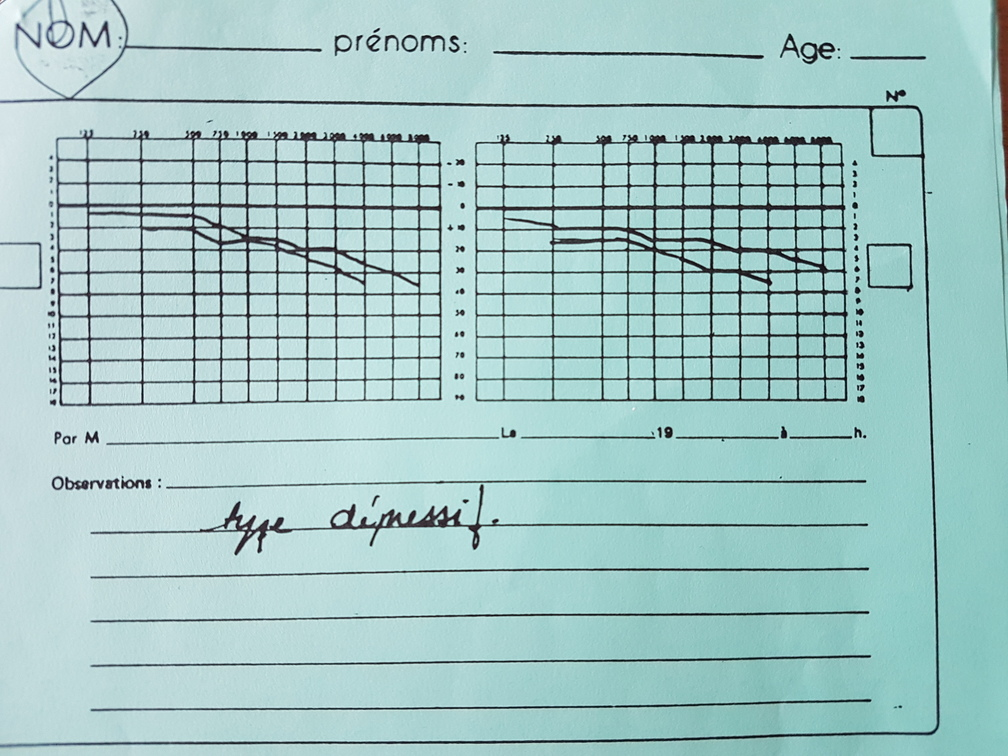
\includegraphics[width=0.7\linewidth]{images/courbedepressif.jpg}
	\caption[Exemple d'une courbe de dépressif]{Courbe classique représentative du dépressif}
       
	\label{groupecontroleimage1}
\end{figure}




  

\paragraph{Le corps et le psychisme}

``\emph{l'alliage indissociable du corps et du psychisme, 
visible et lisible, résultat de l'écoute de sons.''}\footnote{\emph{Extrait de l'entretien Tomatis réalisé par Auriol, Anvers 1973}}



\section{Interprétation: les 3 zones de fréquences avec leur résonance en musicothérapie et en
  psychologie}


	Informations croisées avec les informations récoltées par les 3 
          zones du test d'écoute:
          
Les paramètres utilisés en musicothérapie trouvent leur lien avec les
3 zones de fréquences d'interprétation psychologique du test d'écoute.
\begin{itemize}
 \item Le rythme, tempo, puls  =  Z.1: le physique, le corps, l'incorporéisation et
l'intégration du rythme,
la posture d'écoute.

\item La voix, le timbre, la mélodie =  Z.2:  l'expression vocale, la communication,
l'émotionnel, la sensibilité, l'affect.

\item La justesse= l'harmonie (consonance, dissonance) et l'improvisation = Z.3:  la créativité, l'interprétation, la
résonance, la musicalité, la motivation, le non-verbal (
l'intraduisible en mot), l'espace.
\end{itemize}
A cette interprétation graphique, nous pourrions renchérir nos
observations avec les relations
qu'E.
Willems  avait établies entre vie humaine et vie musicale, c.à.dire
\begin{itemize}
  \item vie corporelle (impulsions physiques-----vie rythmique
  \item vie affective (émotions, sentiments)------vie mélodique
    \item vie mentale (raisonnement, intellect-----vie harmonique
\end{itemize}

Si nous référons à la conception antique des chakras ainsi qu'au sens de la
topique de Freud (ça, moi et surmoi), nous trouvons également des correspondances
avec les trois zones entre les
fréquences et ``la distribution de l'énergie pulsionnelle'' ou entre
les 
``caractéristiques du son et l'énergie instinctuelles''. (B.Auriol, La
clef des sons).
``La mélodie est la seule forme musicale de la décharge individuelle, car le rythme est le moteur, pré-musical, et l'harmonie, supra-individuelle `` (Mosonyi, 1935, cité par Michel, 1965).
Pour compléter encore le concept de la zone 3, nous pourrions
également faire un parallèle avec Winnicott et son ``objet
transitionnel'' , le jeu , la capacité de créer un espace
intermédiaire par l'invention, la recherche et ce aussi entre le ``le
dehors et le dedans'' que nous serions tentés, et ce n'est qu'une
hypothése, de de relier à l'interprétations de la courbe aérienne et osseuse de Tomatis. 
 

\begin{figure}
	\centering
	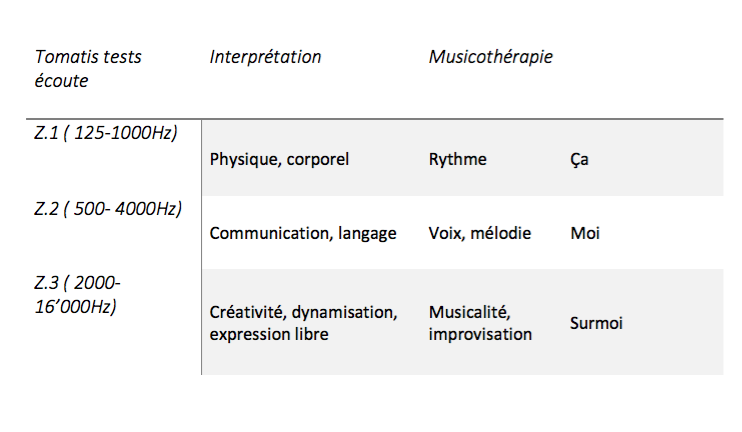
\includegraphics[width=0.7\linewidth]{images/testinterpmusico}
	\caption[ L'interprétation des 3 zones et leur correspondance
        en musicothérapie]{Graphique. interprétation des 3 zones du
          test et leur correspondance en musicothérapie}
       
	\label{graphiquecolonnetestmusico}
      \end{figure}












      


  

\section{Comparaison de deux tests d'écoute, avant et après la musicothérapie: 1°Test--2°test, considérations générales}
	
        \begin{enumerate}
             
        \item Recherche de correspondance entre le premier test d'écoute et
     le premier questionnaire: Il nous a été possible de faire une
     correspondance entre le graphique et le questionnaire en début de
     séjour:


     
     
        \item Comparaison avec 2 tests d'écoute pour chaque individu,
          avant/après séjour pour les deux groupes:
          Observation d'une modification du tests d'écoute:


          
        
        \item\textbf{ Comparaison du 2ème test d'écoute pour GC et GM}
          Nous trouvons avec les deux groupes ayant les mêmes
          pathologies et nous allons observer s'il y a une différence
          dans leur écoute.
\end{enumerate}
	
\subsection{Un cas clinique: Le patient M avant musicoth.}

 	Le patient M souffre de Burnout. Vif, il se montre très
        intéressé pour participer à l'étude.
 
 	
 	\begin{figure}[tbh]
 		\centering
 		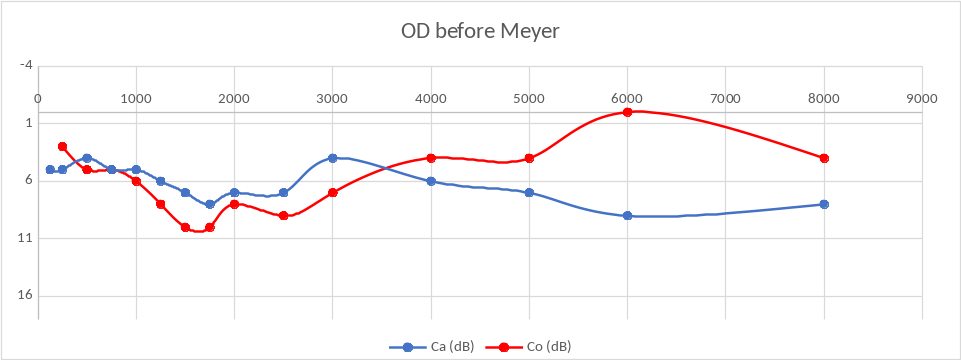
\includegraphics[width=0.7\linewidth]{images/clinique/od_before_meyer.png}
 		\caption{Test d'écoute avant musicothérapie}
 		\label{fig:odbeforemeyer}
 	\end{figure}
 	
 	
 	
 	
 	
 	
 	\begin{figure}
 		\centering
 		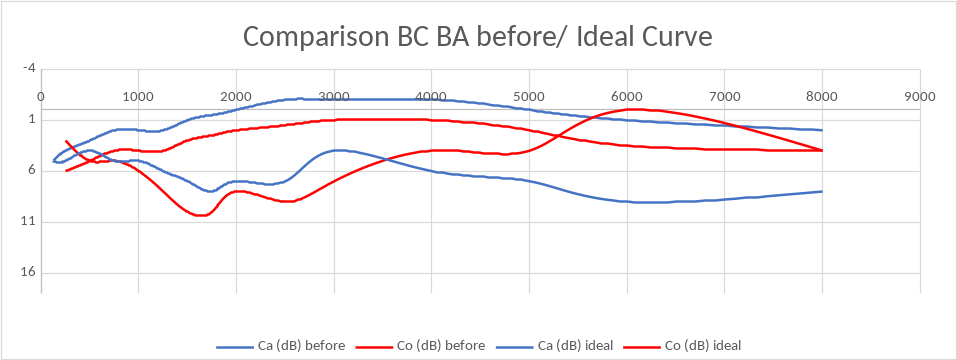
\includegraphics[width=0.7\linewidth]{images/clinique/comparison_bc_ba_before_vs_ideal_curve_meyer.png}
 		\caption[Comparaison avec la courbe idéale]{Comparaison avant
                  musicothérapie des
                  courbes  avec la courbe idéale}
 		\label{fig:comparisonbcbabeforevsidealcurvemeyer}
 	\end{figure}
 	
 	
 	\subsection{Le patient M après la musicoth.}
 	\lipsum[1]
 	\begin{figure}[h]
 		\centering

 		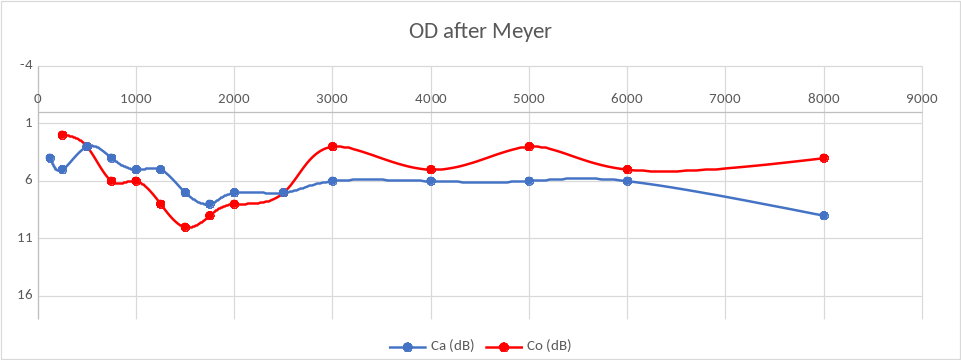
\includegraphics[width=0.7\linewidth]{images/clinique/od_after_meyer.png}
 		\caption{Test d'écoute après la musicothérapie}
 		\label{fig:odaftermeyer}
 	\end{figure}
 
 \lipsum[1]
 
 \begin{figure}[bh]
 	\centering
 	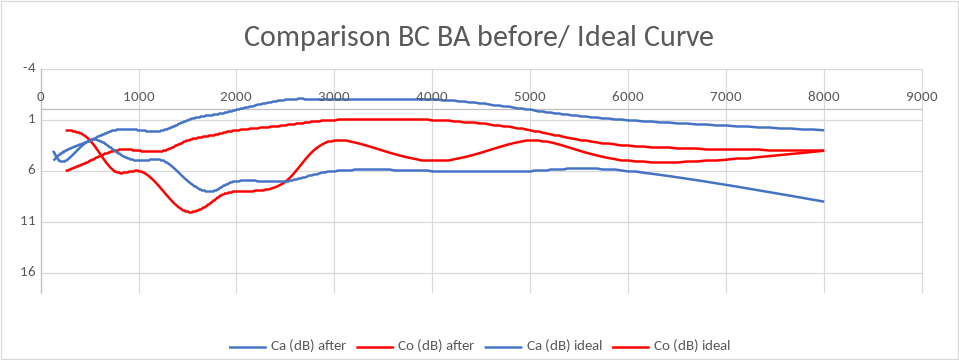
\includegraphics[width=0.7\linewidth]{images/clinique/comparison_bc_ba_after_vs_ideal_curve_meyer.png}
 	\caption{Comparaison avec courbe idéale, après}
 	\label{fig:comparisonbcbaaftervsidealcurvemeyer}
 \end{figure}
 
 





      



 


\section{Graphique:  WHOQO-Bref et Test d'écoute}

Le patient 


\section{Résultats}










   
 

  

  
  


   
   
   
   







\paragraph{Hypothèse}



\paragraph{Y-a-t-il une modification de l'écoute du patient après une prise
en charge en musicothérapie ?}
Est-ce que le processus d'écoute en musicothérapie améliore la capacité
d'écoute ? Devient-elle différente après une musicothérapie?

Est-ce que les test auditifs avant et après la musicothérapie permettent
de visualiser l'action de la musicothérapie?


\paragraph{Est-ce que les résultats ($=$ un changement dans l'écoute) d'une prise
en charge musicothérapeutique peuvent être lisibles et visibles dans
un test d'écoute?}
Est-ce possible d'évaluer un travail musicothérapeutique au moyen
d'un test d'écoute?
Est-ce que ces résultats sont significatifs? 

\paragraph{Est-ce que l'écoute du patient s'est modifié ? si on a pu observer
une modification, dans quel sens va -t-elle ?}

Le contexte: 
est-ce que le contexte est suffisant pour
ressortir des résultats ?





